\documentclass[pdftex,12pt]{artikel3}   

% Settings for source listings.

\usepackage[dvips,letterpaper,margin=1.1in]{geometry}
\usepackage{listings,graphicx}
\usepackage{url,hyperref}     % creates a lot of warning messages...

\lstset{tabsize=2,language=Python,showstringspaces=false}

\title{Informatike I \hfill CSCI-141\\
Vizatimet e breshkes \hfill Leksion 1}
\author{} % \author{RIT CS1 group} 
% revised bks 07/06/17 to revise faculty section and reword implementation
% revised bks 01/16/17 to add done() to the companion code and faculty notes
% revised bks 07/10/13 to change to csci141
% revised atd 08/24/12 to remove pseudocode
\date{}   % \date{09/01/2011} 

\begin{document}
\vspace{-27mm}
\maketitle

\vspace{-27mm}
\begin{tiny}
\hfill \date{08/17/2017}
\end{tiny}
\vspace{-6mm}

\section{Pershkrimi i problemit}

\begin{center}
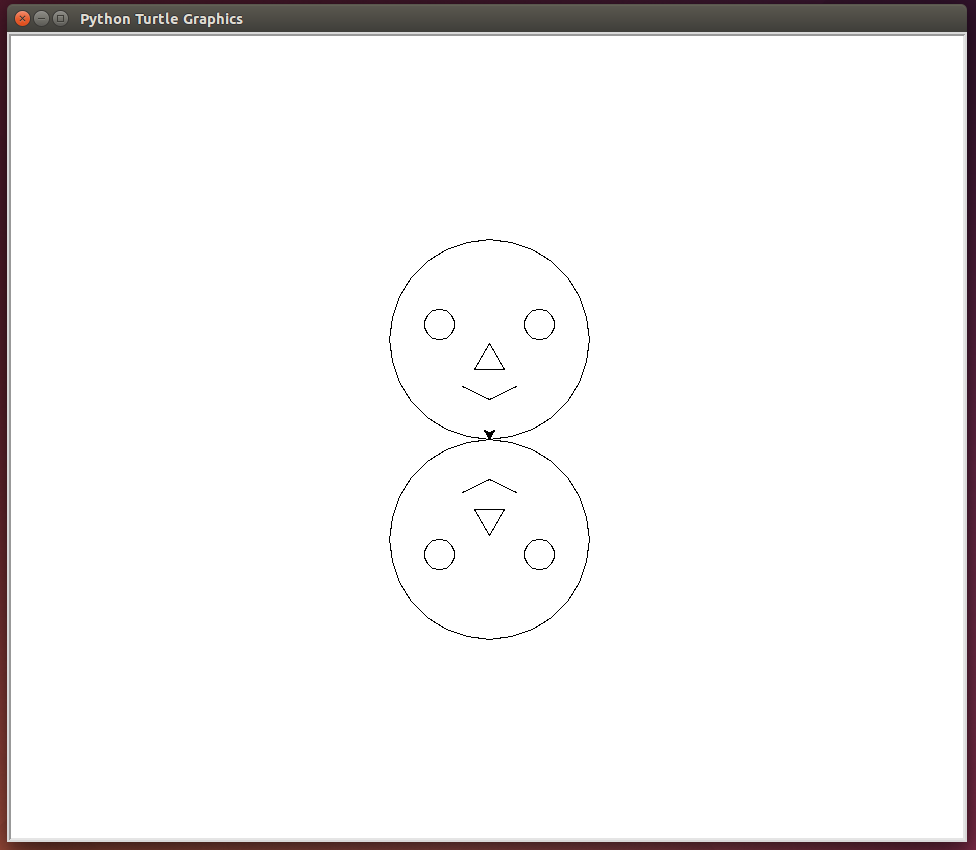
\includegraphics[width=3.0in]{Faces.png} 
\end{center}

Nje menyre per te bere vizatime te thjeshta eshte duke perdorur librarine \texttt{turtle} ne Python. Si fillim, le 
te shikojme si mund te vizatojme nje fytyre. Per te nenvizuar "riperdorimin" e programeve, ne kete rast do vizatojme dy fytyra.
% Using Python's turtle graphics module, we would like to design a
% program that draws a simple face, worthy of a stick figure.  To
% emphasize ``code reuse,'' the program will ultimately draw two faces.


\section{Analiza dhe projekti i zgjidhjes}

Komandat e perdorura jane pjese te librarise turtle. Breshka (turtle) eshte nje objekt imagjinar qe leviz ne hapesiren 
e ekranit dhe ka ne dore nje laps. Gjate levizjes breshka mund te vizatoje figura te ndryshme. Disa nga veprimet jane:
% We will utilize commands commonly found in turtle drawing packages. 
% Turtles are small imaginary objects that have pens 
% connected to their undersides. 
% Examples of what the turtle can be told to do include:
\begin{itemize}
\item ecje para per nje distance te caktuar;
% move forward or backward a certain distance;
\item levizje rrethore (ne drejtim te kundert me akrepat e ores);
% move in a circle (Python always draws them counter-clockwise (CCW));
\item rrotullim majtas (djathtas) me nje numer te caktuar gradesh;
% turn a certain number of degrees left (CCW) or right (CW);
\item ulje/ngritje e lapsit. Kur lapsi eshte poshte, cdo levizje e breshkes vizatohet ne ekran. 
% put its pen up or down. If its pen is down, 
%the turtle will draw a line as it moves, revealing its path.
\end{itemize}

% Our design will involve these activities:
Projekti i zgjidhjes perfshin keto aktivitete:
\begin{itemize}
\item Percaktimi i nje pozicioni fillestar (home) per breshken.
%Define a \emph{home position} for the turtle.
\item Pershkrim ne menyre algoritmike i levizjeve qe i duhen breshkes per te vizatuar figuren e kerkuar dhe per tu kthyer 
ne pozicionin fillestar.
% Describe, via \emph{algorithms}, 
%how to draw each feature of the face by leaving the home position, 
%drawing the feature, and then returning to the home position.
\end{itemize}

{\bf Pozicioni fillester}: Mesi i ekranit, me breshken qe shikon drejt veriut (V)
dhe me lapsin e ngritur lart.
% with the turtle facing upward (“North”)
% and its pen up is the desired home position for this problem.

Duke percaktuar nje pozicion fillestar eshte me e lehte te shtosh ose te heqesh pjese nga figura.

% By defining a home position, we make it easier to add, remove, or 
% rearrange the order of the feature-drawing algorithms.
% This flexibility has a cost:
% the extra movement from and to the home position causes
% our design to be somewhat less efficient than a brute force design.
% Flexibility of design and performance/efficiency are software qualities 
% that are often at odds.

%% While the extra movement to and from the home position does
%% make the design somewhat less time-efficient than a brute force design,
%% this adds flexibility to the solution.
%% Flexibility of design and efficiency/performance are software qualities that are quite often at odds.

\subsection{Algorithms}

An \emph{algorithm} is a special set of instructions.
In the words of David Berlinski\footnote{{\bf Advent of the Algorithm}.
Harcourt. ISBN 0156013916 / 9780156013918 / 0-15-601391-6.},
\begin{center}
\begin{tt}
An algorithm is

a finite procedure,

written in a fixed symbolic vocabulary,

governed by precise instructions,

moving in discrete steps, 1, 2, 3, ...,

whose execution requires no insight, cleverness, \\

intuition, intelligence, or perspicuity,

and that sooner or later comes to an end.
\end{tt}
\end{center}

Below we define two algorithms.
One will put the turtle in its home position, 
and the other will draw the entire face.
Each algorithm is decomposed into a series of smaller steps.
Executing the whole program consists of calling a procedure to
execute the first algorithm, followed by calling a procedure to
execute the second algorithm. 

{\bf Initialization Algorithm}
\begin{itemize}
\item 
move turtle to home position
\item
rotate turtle north
\item
lift pen up
\end{itemize}

{\bf Face-Drawing Algorithm}
\begin{itemize}
\item
draw the outline of the face
\item
draw the mouth
\item
draw the nose
\item 
draw the eyes
\end{itemize}

\subsection{Implementation}
We will see that for this program
each step of the Initialization algorithm
can be implemented using a built-in command from the turtle drawing package.
The steps of the Face-Drawing algorithm have a 
more elaborate implementation and need to be expanded when
written in Python code.
Each `draw' command of the Face-Drawing algorithm 
exists as a separate function, or procedure, in the solution file.

It's important to have documentation on 
the language and the modules we need to use to solve this problem.
There are a number of links to Python language documentation on the 
course's resources page,
\begin{tt}
	\url{http://www.cs.rit.edu/~csci141/resources.html}
\end{tt}
You may find the ``Summary Sheet'' a good place to start.
Information on the functions and procedures of the turtle module is at
\begin{tt}
	\url{http://docs.python.org/py3k/library/turtle}
\end{tt}

See the accompanying source file, {\tt smiling\_faces2\_py.txt}.
\emph{Note: The file has a {\tt .txt} suffix because
browsers may try to execute Python source files.}

Note: 
When the turtle software is loaded, the turtle is already at the location 
we desire for this program, and it is facing East. 
All we need to do is orient the turtle correctly and pull its pen up.

\section{Testing (Test Cases, Procedures, etc.)}

Large software programs have a practically infinite number of different ways they might execute, depending on input supplied to them. It is quite an art to choose a small set of tests that cover all the functionality in the software. 
Since this program is very small, this is not hard to do.
Here are the two test cases.

\begin{enumerate}
\item
Does a single face get drawn correctly?

Call the Face-Drawing procedure with the turtle 
at its starting position.

\item
Does it draw a face correctly, no matter where the turtle starts, 
and no matter how many times the face-drawing procedure is executed?

Change the turtle's position and orientation and 
call the Face-Drawing procedure again; the program should
draw a new face at that new location and orientation.
\end{enumerate}

\newpage

%% =============================================================
%% faculty notes section
%% =============================================================

\section{Learning Objectives} % \section{Presentation Notes}

There is a lot in this lecture, especially for students with
no experience (and instructors who are new to the course).

Students should learn:
\begin{enumerate}
\item
the details of the course and its operation (web page, syllabus, mycourses);
\item
Python function definition and 
interpretation of `{\tt .py}' files (and at the `$>>>$' prompt);
\item
the concepts of computational problem-solving using an example problem;
and
\item
How to approach and solve a specific problem (drawing faces) using Python.
\end{enumerate}

\subsection{Learned by the End of the Lecture}

By the end of the lecture, the student should be able to:
\begin{itemize}
\item
  Start the Python interpreter, and quit the Python interpreter to terminate.
\item
  Import the Python turtle module
  using either {\tt import turtle} or {\tt from turtle import *}.
  (While the first requires more typing, it is preferred because it 
  enforces the notion of calling a function on an object, which is useful later.)
\item
  Create a {\tt .py} file containing functions with documentation.
\item
  Run a {\tt .py} file to execute its main function.
\item
  Look up information on built-in Python functions and modules.
\item
  Describe simple program flow (statement execution).
\item
  Define and then invoke a parameter-less function.
\item
  Describe the requirement of proper indenting
  and the problem of tabs versus spaces.
\item
  State that they always need to use Python version 3
  (the names end in ``3'' in CS department *NIX machines).
\item
  Use the {\tt input} and output (i.e. {\tt print}) commands.
\end{itemize}

\subsection{Logistics to Learn by the End of the Lecture}

At the end of lecture, make sure the students know the following:
\begin{itemize}
\item
  Where the homework assignment is located, and when it must be uploaded;
\item
  When and where to go for the lab session;
\item
  When and where to go for the recitation session; and
\item
  How they will get their CS department accounts (i.e. from the SLI in lab).
\end{itemize}

\subsection{Problem-specific Learning Details} % \subsection*{Concepts}

\begin{itemize}
\item
  General problem solving techniques
\item
  Graphics programming using a line drawing package
\item
  Pen control routines
    \begin{itemize}
    \item
    Setting the pen position
    \item
    Raising and lowering the pen
    \item
    Moving and turning the pen 
    \item
    Waiting with the {\tt done} versus the {\tt input} commands.
    \end{itemize}
\item
  Testing
\end{itemize}

\subsection{Learning Activities}

\begin{enumerate}
\item
  Describe the course structure, organization and materials.
\item
  Introduce the Python programming language and development environment.
\item
  Introduce a Computational Problem-solving Approach.
\item
  Practice the approach on a specific problem (drawing faces).
\end{enumerate}

The instructor should present the problem in the following order:
\begin{itemize}
\item
  Draw an approximation of the desired figure on the board.
\item
  Go over the Python code (at the procedure level) or develop it live in class.
\item
  List the operations needed, and 
  show their online documentation. Here are some ways:
    \begin{itemize}
    \item
    Use a browser to search and include the search text `\emph{python 3}'
    so that you will get results for Python version 3 instead of version 2.
    \item
    Use {\tt pydoc3 turtle} in a shell.
    \item
    {\tt help( turtle )} in the interpreter (after {\tt import turtle}.
    \item
    Or visit \url{http://docs.python.org/py3k/library/turtle}.
    \end{itemize}
\item
  Ask students to develop the subroutines 
  for drawing different parts of the figure.
\item
  Introduce the Python language (version 3) and the turtle package.
\item
  Go over the implementation or develop it live in class.
\item
  Introduce either the editor \textbf{PyCharm}, \textbf{idle} (version 3)
  or \textbf{vim}, based on (a) whether or not the class uses a PC-based lab
  and (b) instructor's personal preference.
\item
  Verify the solution using the first test case.
\item
  Run the second test case, which draws a second figure 
  at a new position and orientation; all the functions still work properly.
\end{itemize}

\end{document}
